%\documentclass[]{IEEEphot}
\documentclass[conference]{IEEEtran}
\usepackage[utf8]{inputenc}
\usepackage[parfill]{parskip}
\usepackage{tikz}
\usepackage{amssymb}

\usepackage[section] {placeins}
\graphicspath{{src//images//}}

\renewcommand{\labelenumi}{\arabic{enumi}. } % Changes enumerate style to number+dot

%\jvol{xx}
%\jnum{xx}
%\jmonth{November}
%\pubyear{2011}

\begin{document}
\title{Clustering Algorithms Overview}
\author{
	\IEEEauthorblockN{Mater Drame, Primož Bajželj \\ Mentor: Matej Pičulin}
	\IEEEauthorblockA{Faculty of Computer and Information Science, Ljubljana}
}
\maketitle

\begin{abstract}
Have you ever wondered how is it possible that there is advertisement on a web page you
are intersted in? Or how You-tube is offering you videos you are likely searching for? 
One of the techiques used is clustering. In this paper a few of the most known
algorithms are researched and compared to each other.
\end{abstract}

\begin{IEEEkeywords}
k-means, ECM, EMGMM, density, spectral, information theoretic.
\end{IEEEkeywords}

\section{Introduction}
Clustering (or cluster analysis) is an unsupervised machine learning task of partitioning
a dataset into subsets (groups), so that members of the same subset are more similar to each other
(according to some criterion) than to members of other subsets. Each subset is called a cluster.
This task should be accomplished without any prior knowledge about the structure of the data, and in general
even without knowing the number of clusters which comprise the data.

The problem of clustering has been addressed in many contexts and by researchers in many fields. It has
broad appeal and is useful as one of the steps in exploratory data analysis (data mining). The importance
and interdisciplinary nature of clustering is evident through its vast literature and rich history, even
in disciplines such as biology, psychiatry, psychology, archeology, geology, geography and
marketing \cite{jaindubes88}.%[Jain and Dubes, 1988].

Clustering is recognized as an important tool in areas such as image segmentation,
speech recognition, signal compression, medical research, document storage and retrieval,
world-wide-web search and mining as well as bioinformatics.

\begin{figure}[h]
\label{taxonomy}
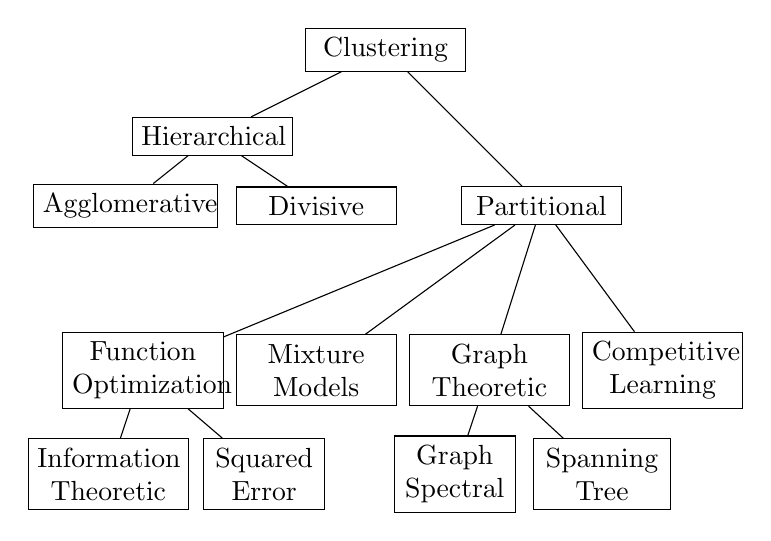
\begin{tikzpicture}[scale=1.1, text width=1.8cm, text centered]
    \tikzstyle{every node} = [rectangle,draw]

    \node (a) at (7, 5) {Clustering};
    \node (b) at (5, 4) {Hierarchical};
    \node (c) at (8.8, 3.2) {Partitional};

    \node (d) at (4, 3.2) [text width=2.1cm] {Agglomerative};
    \node (e) at (6.2, 3.2) {Divisive};

    \node (f) at (4.2, 1.3) {Function \\ Optimization};
    \node (g) at (6.2, 1.3) {Mixture \\ Models};
    \node (h) at (8.2, 1.3) {Graph \\ Theoretic};
    \node (i) at (10.2, 1.3) {Competitive \\ Learning};

    \node (j) at (3.8, 0.1) {Information \\ Theoretic};
    \node (k) at (5.6, 0.1) [text width=1.3cm] {Squared \\ Error};

    \node (l) at (7.8, 0.1) [text width=1.3cm] {Graph \\ Spectral};
    \node (m) at (9.5, 0.1) [text width=1.5cm] {Spanning \\ Tree};

    \draw [-] (a) -- (b);
    \draw [-] (a) -- (c);

    \draw [-] (b) -- (d);
    \draw [-] (b) -- (e);

    \draw [-] (c) -- (f);
    \draw [-] (c) -- (g);
    \draw [-] (c) -- (h);
    \draw [-] (c) -- (i);

    \draw [-] (f) -- (j);
    \draw [-] (f) -- (k);

    \draw [-] (h) -- (l);
    \draw [-] (h) -- (m);
\end{tikzpicture}
\caption{Taxonomy of clustering approaches.}
\end{figure}

Due to ill-posed nature of clustering (the goal is to find a \textit{reasonable} partition of the data),
no clustering technique is universally applicable, resulting in tens, if not hundreds of various algorithms
that differ significantly in their notion of what constitutes a cluster or how to find them.
Figure ~\ref{taxonomy} shows a number of different clustering methods. This taxonomy was given
by \cite{jenssen05}.%[Jenssen, 2005].

The hierarchical clustering algorithms produce $n$ levels of groupings, where $n$ is
the number of examples in data (sometimes called data patterns, feature vectors or observations). These
methods yield a dendogram which represents the similarity levels at which groupings change.
Reader can learn more about these approaches in \cite{kononenko07}. The partitional
clustering algorithms produce a single partition of the data. They often need the number of clusters
to be specified in advance but are usually more computationally efficient.

% TODO: related work (Jain)

In this article we discuss several clustering algorithms, from the most intuitive and most commonly
used k-means through more advanced Expectation Maximization and density-based algorithms
to some newer developments such as spectral clustering and information theoretic clustering.

% TODO: maybe structure of the article?

\subsection{Determining the number of clusters in a dataset}
A major problem in clustering is the fact that many clustering algorithms require the
number of clusters to find in a dataset as input (this quantity is usually denoted $k$).
Several algorithms such as those based on density do not require the specification of this
parameter and hierarchical clustering algorithms essentially output clusterings (a clustering
is simply a set of clusters, usually containing all the data)
for all possible values of this parameter (somewhat avoiding the problem).

The average silhouette of the data is a useful criterion for assessing the number of clusters in data.
The silhouette of an example is a measure of how well matched it is to the cluster it is assigned
and how loosely it is matched to the neighbouring cluster. The average silhouette of a cluster
is therefore a measure of how tightly grouped all the data in the cluster are and the average silhouette of
the entire dataset measures how appropriately the data has been clustered. We can cluster a dataset
several times with different values of algorithm's parameters and then decide which clustering to keep based on
the average silhouette.

The Elbow method looks at the percentage of variance (the ratio of the between-group variance
to the total variance) explained as a function of the number of clusters.
The number of clusters should be chosen so that adding another cluster doesn't give much better modelling
of the data. For example, when clustering with the k-means algorithm, we can compute the sum of square (SS)
distances within clusters as well as the total SS, and look for a large gap in percentage of variance
from one k to the next k+1.

The Calinsky and Harabasz method computes
\begin{equation}
\label{calinsky}
CH(k) = \frac{B(k)/(k-1)}{W(k)/(k-1)}
\end{equation}

where $B(k)$ and $W(k)$ are the between and within cluster sum of squared errors (distances),
with $k$ clusters. The idea is to maximize $CH(k)$ over the number of clusters $k$. In effect, this
is a measure of inter-cluster similarity over intra-cluster similarity.

\section{Clustering performance evaluation}
To compare different clustering algorithms we need to evaluate clustering results (referred to as cluster validation).
A measure of similarity between two clusterings can be used to compare how well different clustering algorithms perform
on a dataset. The literature divides these measures into two large groups: those used for \textit{internal} evaluation
and into \textit{external} evaluation methods. Internal evaluation methods evaluate a clustering result on the data
that was clustered. This evaluation is biased towards algorithms that use the same cluster model. Examples of such methods
include Davies-Boulding index and Dunn index. In external evaluation, clustering results are evaluated based on data
that was not used for clustering, such as known class labels. This usually requires human-created datasets. Rand measure,
Adjusted Rand measure (or index), F-measure, Jaccard index, Fowlkes-Mallows index and Mutual Information are examples
of external evaluation methods. We used ARI, homogeneity and completeness:

\subsection{Adjusted Rand Index}
Rand Index (RI) is a measure of similarity between data clusterings. It counts
the number of agreements between two clusterings:

\begin{equation}
\label{RI}
RI = \frac{a+b}{{n \choose 2}}
\end{equation}

where
\begin{itemize}
    \item \textit{a} is the number of pairs of examples that are in the same cluster in the first clustering
    as well as in the other clustering,
    \item \textit{b} is the number of pairs of examples that are in different clusters in both clusterings,
    \item \textit{n} is the number of elements.
\end{itemize}

Adjusted Rand Index (ARI) is the corrected-for-chance version of RI.
ARI has the advantage over plain RI in that it scores random 
clusterings close to 0 for any number of clusters and data samples. It returns
a value in range $[-1, 1]$, where negative values are bad, similar clusterings have
positive values and 1.0 is the perfect match score. ARI makes no assumption on the cluster
structure and can therefore be used to compare different algorithms such as k-means (which
constructs isotropic clusters) with spectral or other algorithms (which can find non-convex
clusters).

\subsection{Homogeneity, completeness and V-measure}
Rosenberg and Hirschberg \cite{rosenberg07} defined two desirable objectives of clustering: homogeneity and
completeness. Homogeneity refers to a desire that each cluster should contain only members
of a single class whereas completeness expresses the aspiration that all members of a given
class are assigned to the same cluster.
We can translate these objectives to math in the following way:

\begin{equation}
\label{homogeneity}
homogeneity = 1 - \frac{H(C|K)}{H(C)}
\end{equation}

\begin{equation}
\label{completeness}
completeness = 1 - \frac{H(K|C)}{H(K)}
\end{equation}

where $H(C|K)$ is the conditional entropy of the classes given the cluster assignments defined as:

\begin{equation}
\label{hck}
H(C|K) = - \sum\limits_{c=1}^{|C|}\sum\limits_{k=1}^{|K|}\frac{n_{c,k}}{n} \log{\frac{n_{c,k}}{n_k}}
\end{equation}

and $H(C)$ is the entropy of the classes:

\begin{equation}
\label{hc}
H(C) = - \sum\limits_{c=1}^{|C|}\frac{n_c}{n} \log{\frac{n_c}{n}}
\end{equation}

with $n$ the total number of examples, $n_c$ and $n_k$ the number of examples belonging to class
$c$ and cluster $k$ respectively, and with $n_{c,k}$ the number of examples from class $c$ assigned
to cluster $k$.

The conditional entropy of clusters given class $H(K|C)$ and the entropy of clusters $H(K)$ are
defined in a symmetric manner. The same paper defined V-measure as the harmonic mean of homogeneity and completeness:

\begin{equation}
\label{v}
v = \frac{2hc}{h+c}
\end{equation}

Advantages of these measures are bounded scores ($[0, 1]$, 1.0 means perfect score), intuitive interpretation and that
no assumption is made on the cluster structure (similar to ARI). Unfortunately, they are not normalized
with respect to random clustering: random clustering will not yield the same values and it won't
yield zero score when the number of clusters is large compared to the number of examples. For smaller
datasets or larger number of clusters it is better to use an adjusted measure such as ARI.

\section{Algorithms}
\subsection{k-means}
k-means clustering (KMC) is a simple and well known algorithm. It is usually very
fast (commonly run multiple times with different starting conditions), but tends
to produce spherical clusters with similar size, which can be undesirable.
k-means is often used as a preprocessing step for other algorithms. The standard
algorithm was first proposed by Stuart Lloyd in 1957 and published later in 1982.

%The number of clusters we want to find in data is fixed a priori ($k$).
KMC requires as input the number of cluster we want to find in data ($k$).
The algorithm iteratively refines clusters' locations (guided by a cost function),
until no more refinements are possible (clusters do not change anymore)
or max number of iterations has been reached. It can be summarized as \cite{jain00}:

\begin{enumerate}
    \item Select an initial partition with k clusters.
    \item Generate a new partition by assigning each example to its closest cluster center.
    \item Compute new cluster centers as the centroids of the clusters.
    \item Repeat step 2 and 3 until convergence.
\end{enumerate}
%$m_1^{(1)}$, $m_2^{(1)}$, ..., $m_k^{(1)}$
%denote centroids (also called means). The superscript index denotes the current iteration.
%$S_i^{(t)}$ is a cluster (set of examples) with the corresponding centroid $m_i^{(t)}$.
%There are two alternating steps in the algorithm:

%\begin{itemize}
%\item \textbf{Assignment step}\\
  %Each example is assigned to the cluster with the closest centroid:\\
  %$S_i^{(t)} = \{x_j : ||x_j - m_i^{(t)}|| \le ||x_j - m_l^{(t)}|| \forall l = 1, ..., k\}$
%\\
%\item \textbf{Update step}\\
  %New means are calculated and set as centroids:\\
  %$m_i^{(t+1)} = \frac{1}{|S_i^{(t)}|} \displaystyle\sum\limits_{x_j \in S_i^{(t)}}{x_j}$
%\end{itemize}

There are two common ways to select the initial centroids: random seed and random partition.
The random seed method randomly chooses k observations from the dataset
and uses these as the initial means. Random partition
assigns each example into one of the k clusters randomly.
The random seed method tends to spread the initial means out, while random partition
places all of them close to the center of the dataset.

There are also better approaches to initialization: \textit{k-means++} algorithm specifies a
procedure to initialize the cluster centers before proceeding with the standard k-means
optimization iterations. With the k-means++ initialization, the algorithm is guaranteed
to find a solution that is $O(\log k)$ competitive to the optimal k-means solution.
Although this initial selection takes extra time, it speeds up the convergence and 
therefore actually lowers overall computation time.

Although it can be proved that the KMC algorithm will always terminate (converge),
it does not necessarily find the most optimal configuration,
corresponding to the global objective function minimum. The algorithm is also sensitive
to the initial selected cluster centroids but it can be run multiple times to reduce this effect.

Another interesting fact is that, in the worst case, k-means can be very slow to converge:
in particular it has been shown that there exist certain datasets,
even in 2 dimensions, on which k-means takes exponential time to converge.
These datasets do not seem to arise in practice: this is supported by the
fact that the smoothed time complexity of k-means is polynomial.

% TODO: k-medoids

\subsection{Evolving Clustering Method}

ECM (Evolving Clustering Method) is a dynamic clustering method used mostly as a fast \textit{one-pass} online algorithm. % with fast \textit{one-pass} method.
Its extension ECMc (Evolving Clustering Method with Constrained minimization) is used as offline algorithm where constrained optimization
is applied. Both ECM and its extension were introduced in 2001 by Qun Song and Nikola Kasabov \cite{song01}.

ECM is a distance based clustering method where the distance between each of cluster's members and the cluster center is less than $D_{thr}$.%all of cluster's members are less distant
%from the center than $D_{thr}$.
$D_{thr}$ is by default the algorithm's input, unlike to some other algorithms where the number of clusters is required as
input. $D_{thr}$ does affect the number of clusters, but not directly. Therefore, when comparing ECM algorithm to
others, we have to be aware of their inputs.

The algorithm takes examples from a data stream and proceeds with one of three actions: updating corresponding cluster radius, changing
cluster center or creating a new cluster.
%every new data cluster's radius can be updated or it's center changed or
%new cluster can be created.
At some point, usually when cluster radius reaches threshold value $D_{thr}$, cluster radius
is not updated anymore.

Both ECM and ECMc consist of several steps where ECM is a preprocess to ECMc. First example is used to create the first cluster
with radius 0 and center on the example itself. For every new example $x_i$ these next steps are taken:
\begin{enumerate}
	\item Distance from $x_i$ to every cluster center is calculated as shown in equation \ref{ECMdist}.
	\item If minimum distance found is less than or equal to cluster radius, $x_i$ belongs to cluster and algorithm returns to step 1.
	\item For every cluster s is calculated as shown in equation \ref{ECMequ1}. If minimum s is more than $2*D_{thr}$ a new cluster
		is created and algorithm continues at step 1.
	\item Cluster's center, with minumum s calculated, is moved and radius increased. New radius is calculated as $s/2$ and
		center's position is on the line from the old center to the example $x_i$ so that distance from the new center to the example $x_i$ is
		equal to $s/2$ as shown in equation \ref{ECMequ2} and \ref{ECMequ3}.
\end{enumerate}

\begin{equation}\label{ECMdist}
dist(i,j) = \sqrt{ \frac {\sum_{d=1}^{D} (x_i^d - C_{cj}^d)^2} {D}}
\end{equation}

\begin{equation}\label{ECMequ1}
s(i, j) = dist(i,j) + radius(C_j)
\end{equation}

\begin{equation}\label{ECMequ2}
f = 1 - \frac {\frac {s} {2}} {\sqrt{ \sum_{d=1}^{D} (C_c^d - x_i^d)}}
\end{equation}
\begin{equation}\label{ECMequ3}
Cc^d = Cc^d + (f \cdot (x_i^d - C_c^d))
\end{equation}

%This way it holds for each example in its own cluster that the distance between the center and the example
%is less than or equal to $D_{thr}$.
As a result, distances between examples and their corresponding cluster centers are less than or equal to $D_{thr}$.
Afterwards, constrained optimization can be applied to minimize the function \ref{ECMJ}. For optimization the following steps have to be taken:
\begin{enumerate}
	\item Change the membership of each example to a cluster that has the smallest distance to its center.
	\item Calculate new cluster center to satisfy changes.
	\item Algorithm terminates if enough iterations occured or the value of \ref{ECMJ} changed less than a certain amount.
		Otherwise return to step 1.
\end{enumerate}

\begin{equation}\label{ECMJ}
	J = \sum_{k=1}^K \sum_{i=1}^{N_{Ck}} dist(x_{ki}, C_{ck})
\end{equation}


\subsection{Expectation Maximization Gaussian Mixture Model}

Gaussian Mixture Models are among the most statistically mature methods for clustering. Unlike k-means,
GMMs are able to build soft clustering boundaries, i.e., examples can belong to any class (cluster) with a given probability.

For statistical models Gaussian distribution is mostly used, in which parameters are the mean vector $\mu$ and a
variance-covariance matrix $\sum$. Its probability density function is shown in equation \ref{equgauss}.

\begin{equation}\label{equgauss}
	N(x|\mu,\sum) = \frac{1}{\sqrt{(2\pi)^D \cdot |\sum|}} \cdot e^{-\frac{(x-\mu)^T \cdot \sum^{-1} \cdot (x-\mu)}{2}}
\end{equation}

Because one distribution cannot accurately model all the data we use a mixture of distributions - convex
combinations of more probability distributions. Mixture distributions have an array of component distributions
($\mu$,$\sum$) and a coefficient array ($\pi_k$), which contains the weight of each component's probability distribution
as shown in equation \ref{equmixdist}.

\begin{equation}\label{equmixdist}
	p(x) = \sum_{k=1}^K {\pi_k N(x|\mu_k, {\sum}_k)}
\end{equation}

Three parameters $\pi$, $\mu$ and $\sum$ have to be defined to suit the maximum likelihood as in the equation \ref{equmaxlike}
and \ref{equmaxlike2}.

\begin{equation}\label{equmaxlike}
	MLE=\arg\max_\theta {p(P|o)} = \arg\max_\theta {p({x1,x2,...,xn}|\pi,\mu,\sum)}
\end{equation}
\begin{equation}\label{equmaxlike2}
	MLE = \arg\max_\theta {\prod_{i=1}^N p(x_i|\pi,\mu,\sum)}
\end{equation}

The problem can be simplified by taking the log of the function that gives us huge advantage of converting the
product into a sum as shown in equation \ref{equmaxlikelog}.

\begin{equation}\label{equmaxlikelog}
	MLE=\arg\max_\theta {\sum_{i=1}^N log(p(x_i))}
\end{equation}

Taking the derivative of the likelihood function with respect to $\mu$ and setting the result to 0, $\mu$ can be found as
shown in equation \ref{equfindmi}, \ref{equrik}. Similarly, if we take derivative with respect to $\sum_k^{-1}$ and set
result to 0 we get $\sum_k$ shown in equation \ref{equsumk}. For $\pi_k$ we take derivative of $\pi_k$ and get equation
shown in \ref{equpik}.

\begin{equation}\label{equfindmi}
	\mu_k = \frac {\sum_{i=1}^N r_{ik} x_i} {\sum_{i=1}^N r_{ik}}
\end{equation}
\begin{equation}\label{equrik}
	r_{ik} = \frac {\pi_k N(x_i|\mu_k,{\sum}_k)} {\sum_{j=1}^K \pi_j N(x_i|\mu_j,{\sum}_j)}
\end{equation}
\begin{equation}\label{equsumk}
	 {\sum}_k = \frac {\sum_{i=1}^N r_{ik} (x_i-\mu_k) (x_i-\mu_k)^T} {\sum_{i=1}^N r_{ik}}
\end{equation}
\begin{equation}\label{equpik}
	\pi_k=\frac {\sum_{i=1}^N r_{ik}} {N}
\end{equation}

We also introduce hidden variables $s_i$ that define if an example belongs to a certain group.

Using Expectation Maximization we numerically find the solution. Algorithm got its name from steps E and M,
which are essential. In step E we calculate the values of hidden variables $s_i$ and in step M we correct the parameters based
on the values of hidden attributes. Steps to follow:

\begin{enumerate}
	\item All parameters, means, convariances and mixing coefficients, have to be set and the initial value of log-likelihood
		function has to be evaluated.
	\item Values of $r_ik$ should be calculated based on set parameters.
	\item New values of means, covariances and mixing coeficients should be evaluated with $r_{ik}$ in step 2.
	\item Log-likelihood function should be calculated again and checked for convergence. If threshold convergence
		is not reached we continue at step 2.
\end{enumerate}


\subsection{Density-based clustering}
This is a group of algorithms which define clusters as areas of higher density than the rest
of the dataset. Examples in sparse areas in between clusters are considered noise. The notion
of noise actually particulary sets these algorithms apart from others.

The best known density-based clustering method is DBSCAN, proposed by \cite{ester96}.
DBSCAN searches neighborhoods (according to some distance measure) of examples,
counting the neighbors (to some distance). If a
particular neighborhood contains sufficiently many examples, the entire neighborhood is
designated to belong to a new cluster. The algorithm then searches the neighborhoods of examples
in this new cluster, expanding it until it is completely found.
This process is repeated with random unassigned examples until no new clusters can be started.
Examples which were not assigned to clusters are classified as noise.

The time complexity of DBSCAN is most affected by the neighborhood queries. If a spatial
indexing structure is used to provide logarithmic queries, then the overall time complexity
is $O(n\log n)$. Advantages include the ability to find arbitrarily shaped clusters (even
non-linearly separable ones, which cannot be clustered with e.g. k-means); it has a notion of
noise and does not require the specification of the number of cluster in advance (since it
discovers clusters naturally by itself). However, it has difficulties handling data containing
clusters of different densities and is very sensitive to input parameters (e.g. setting
the neighborhood search distance too low might result in classifying examples as noise
rather than aggregating them into a cluster). It also fails on overlapping clusters such as
those in mixtures of Gaussians (where EM clustering is superior).

Hierarchical clustering algorithm Chameleon \cite{karypis99} builds a list of the nearest
neighbors of each example, constructs a weighted similarity graph (described in Spectral clustering)
using this nearest neighbor list, and then partitions the graph to obtain cluster fragments
which are finally merged into clusters. It is similar to DBSCAN in that it finds a small subsets
of examples and builds clusters around them. Chameleon can handle clusters of varying density,
partly because of its nearest neighbor approach, which tends to work better than distance measures,
especially in high dimensional datasets.

Another hierarchical algorithm CURE \cite{guha98} represents each cluster by a certain
number of examples selected from the cluster and translated toward the mean of the cluster
by a specified amount (this helps with outliers). The algorithm merges clusters with
the closest pair of representative examples at each step. Using more than one representative
example per cluster allows CURE to adjust to non-spherical shapes of the clusters.
CURE also has problems with clusters of different densities \cite{ertoz03}. Its running
time is $O(n^2)$ but the authors of the algorithm used several enhancements such as
random sampling and partitioning to make it more practical.

The SNN algorithm \cite{ertoz03} differs from DBSCAN mainly in that it defines the similarity
between two examples in terms of how many nearest neighbors the two examples share.
Using this new definition of similarity, it eliminates noise and problems with varying density.
It also uses the concept of representative examples which handles problems with shape
and size of clusters. The run-time complexity is $O(n^2)$ since the algorithm constructs
the similarity matrix (can be reduced to $O(n \log n)$ for low dimensional data by using a spatial
indexing structure, such as kd-tree).

% TODO: OPTICS maybe?

\subsection{Spectral Clustering}
Spectral clustering has become more popular in recent years. It uses standard linear algebra
methods, it is relatively simple to implement and its results are often better than those of
traditional clustering approaches (such as k-means). In short, spectral clustering exploits the
eigenvalues and eigenvectors (called spectrum of a matrix, hence the name) of the similarity matrix
(which represents
a measure of similarity between examples) of the data to perform dimensionality reduction for
clustering in low-dimensional space. It is not obvious to see why it works at all
and we will not dive into details in this article, instead we will try to give a high level overview.
An intuitive explanation from three different theoretic backgrounds is given by \cite{luxburg07}.

Similarity graphs and graph Laplacians are the key tools in spectral clustering.
Similarity graph is constructed from data by interpreting examples as vertices and similarities
between examples as weighted edges between vertices. This enables reformulating the problem
of clustering: we want to find a partition of the graph such that the edges between different groups
have low weights (dissimilar examples) and the edges within a group have high weights (similar examples).
There are several ways of building these graphs:
\begin{itemize}
    \item $\epsilon$-neighborhood graph: All examples whose pairwise distances are smaller than $\epsilon$
    are connected. In practice it can be difficult to choose a useful value for $\epsilon$. Setting it too
    low might fail to connect sparse clusters, whereas setting it too high might unnecessarily connect many
    examples (different scales problem).
    \item $k$-nearest neighbor graph: Each example is connected with its nearest $k$ examples. Recommended
    by \cite{luxburg07}.
    \item Fully connected graph: Simply connecting all examples with each other. Results in a dense matrix.
\end{itemize}

% TODO: connection with graph cut!

Graph Laplacian matrices are studied in Spectral graph theory. They encode graph adjacency information
as well as information about degrees of vertices and have some interesting properties used in spectral
clustering, e.g. the multiplicity of the eigenvalue 0 equals the number of connected components in the graph
\cite{mohar91,mohar97}.

There are several variants of spectral clustering algorithms. We will describe only unnormalized version
as presented in \cite{luxburg07}. Given similarity matrix $S \in \mathbb{R}^{n \times n}$ and the number
of clusters to construct $k$:

% TODO: refer to authors of different variants

\begin{enumerate}
    \item Construct a similarity graph.
    \item Compute the unnormalized Laplacian L.
    \item Compute the first $k$ eigenvectors $u_1, \dots, u_k$ of $L$ and combine them into
    $U \in \mathbb{R}^{n \times k}$ as columns.
    \item Cluster rows of $U$ ($y_i \in \mathbb{R}^k$ is the $i$-th row) with the k-means algorithm
    into clusters $C_1, \dots, C_k$.
    \item Output are clusters $A_1, \dots, A_k$, where $A_i = \{ j|y_j \in C_i \}$
\end{enumerate}

The main trick of this algorithm is to change the representation of the examples to $y_i \in \mathbb{R}^k$.
In this new representation clusters can be easily detected, even by a simple algorithm such as k-means.

Spectral clustering is being given a lot of attention mainly because it does not make strong
assumptions on the form of the clusters. Unlike many other clustering algorithms it
can solve very general problems like intertwined spirals.
Spectral clustering can be implemented efficiently even for large datasets, as long as
the similarity graph is sparse. Once the similarity graph is chosen, a linear problem needs to
be solved. There are no issues of getting stuck in a local minima and there is no need to
restart the algorithm several times with different initializations. However, choosing
a good similarity graph is not trivial, and spectral clustering can
be quite unstable under different choices of the parameters for the neighborhood graphs.

Spectral clustering is a newer line of research in otherwise surprisingly old branch of clustering
approaches called graph-theoretic clustering. The best known graph-theoretic algorithm is
based on construction of the minimal spanning tree of the data \cite{zahn71}, and then deleting
the edges with the largest lengths to generate clusters. For an appropriately constructed minimal
spanning tree, this algorithm can handle a wide variety of data structures.

\subsection{Information Theoretic Clustering}%Cauchy-Schwarz Divergence Clustering}
KMC and similar are examples of so-called \textit{parametric} methods of clustering. These
methods assume some knowledge about clusters' structure, which makes them less
suitable for many use cases. KMC performs badly when clusters are not hyperelliptical
because it implicitly assumes Gaussian cluster distributions. In fact, any clustering method
that utilizes second order data statistics can produce only convex clusters \cite{jain00}.

Information theory has been successfully used in clustering by several researchers in recent years.
Various information-theoretic clustering metrics, such as entropy, mutual information and
Kullback-Leibler divergence were researched.

Faivishevsky and Goldberg \cite{faivishevsky10} suggested an algorithm based on maximizing the mutual information
between examples and clusters. Their method does not impose any parametric model on the cluster
distribution because they used a non-parametric estimation of the average cluster entropies (MeanNN,
by the same researchers \cite{faivishevsky09}). Their algorithm starts with random partitioning and continues
with reassigning examples between clusters, trying to improve the cost function they developed,
until improvements become sufficiently small. Algorithm's overall computational complexity is
$O(n^2)$, but it is able to cluster non-convex datasets.

Another group of algorithms was developed by \cite{jenssen03,jenssen05}. They combined
the Renyi entropy \cite{renyi61}, which is an information theoretic measure of uncertainty of a random variable,
and the well known Cauchy-Schwarz inequality, forming Cauchy-Schwarz pdf (probability density function)
divergence measure (statistical distance). The measure between two cluster pdf's $p(x)$ and $q(x)$ is defined as:

\begin{equation}
\label{CS}
D_{CS}(p, q) = -\log \frac{\int p(x)q(x)dx}{\sqrt{\int p^2(x)dx \int q^2(x)dx}}
\end{equation}

This divergence can be regarded as an approximation of Kullback-Leibler divergence between two pdf's \cite{jenssen03}.
An intuitive reasoning behind this measure is that in order to optimize $D_{CS}$, the entropy of each individual cluster must
be small, while at the same time the entropy across the clusters must be large.
Probability density functions can be estimated by a sample-based estimator. Jenssen \cite{jenssen05} used a kernel
density estimator developed by \cite{parzen62} (Parzen-Rosenblatt window technique). This introduces a problem of
choosing the kernel size (this is a problem of all kernel-based methods).

An early idea to maximize the Cauchy-Schwarz pdf divergence was to seed a number
of small initial clusters in the dataset, grow clusters (assigning examples to clusters
in a way that maximizes the divergence) until all examples have been clustered, and then
reassign the members of the worst cluster (decided again by the divergence), reducing the number of clusters. 
The reassigning step is repeated until the desired number of clusters is reached.

Jenssen et at. \cite{jenssen07} derived an optimization procedure based on the technique of Lagrange multipliers.
This resulted in an efficient gradient descent-based clustering algorithm which incorporated kernel annealing
as an optimization strategy. The kernel size may start large during the initial iterations, but then annealed (reduced)
in following iterations. The annealing procedure can also help the algorithm to cope with different data scales,
by discovering large scale structures first, followed by fine tuning as the kernel size is decreased.

The main advantage of these clustering approaches is that the underlying clustering metric is
based on entropy. Entropy conveys information about the shape of probability distribution,
and not only variance (which e.g. k-means rely on). This enables the clustering of datasets consisting of
elongated and highly irregular clusters.

% TODO: connection with graph-theoretic approaches

\section{Results}
We used scikit-learn machine learning library written in Python \cite{scikit}. TODO

\subsection{Datasets}

For each algorithm comparison on three different datasets was done. First dataset shown in picture \ref{dataset1}
represent two clusters that are linear separable. Second one, shown in picture \ref{dataset2},is not linear separable
and that makes it difficult for some algorithms to cluster it correctly. In this second example one
whole cluster is inside another cluster. Next dataset's shape reminds on two half-moons that are hardly seperable.
We can see it on figure \ref{dataset3}.

\begin{figure}[th]
\centering
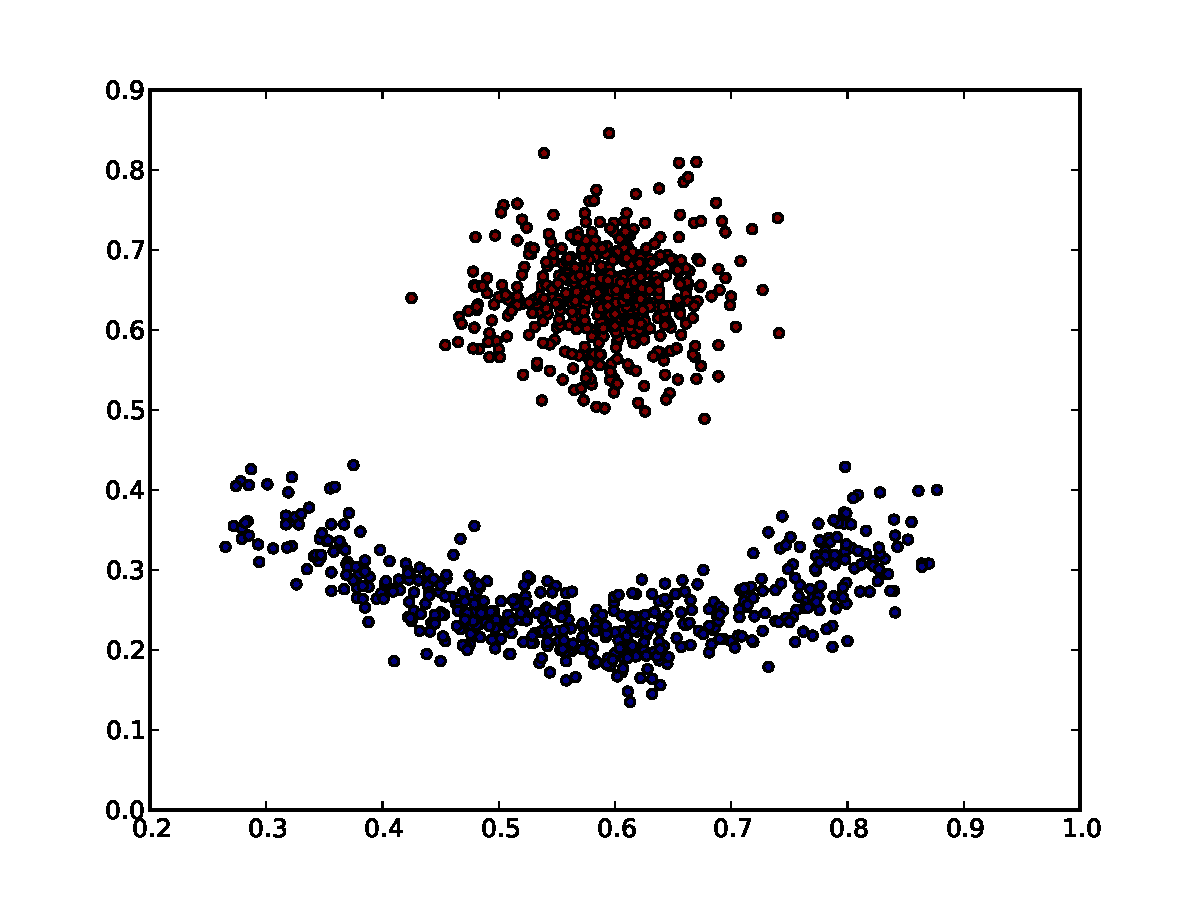
\includegraphics[width=15pc]{red-blue-clusters.pdf}
\caption{Dataset named ''red-blue''.}
\label{dataset1}
\end{figure}

\begin{figure}[th]
\centering
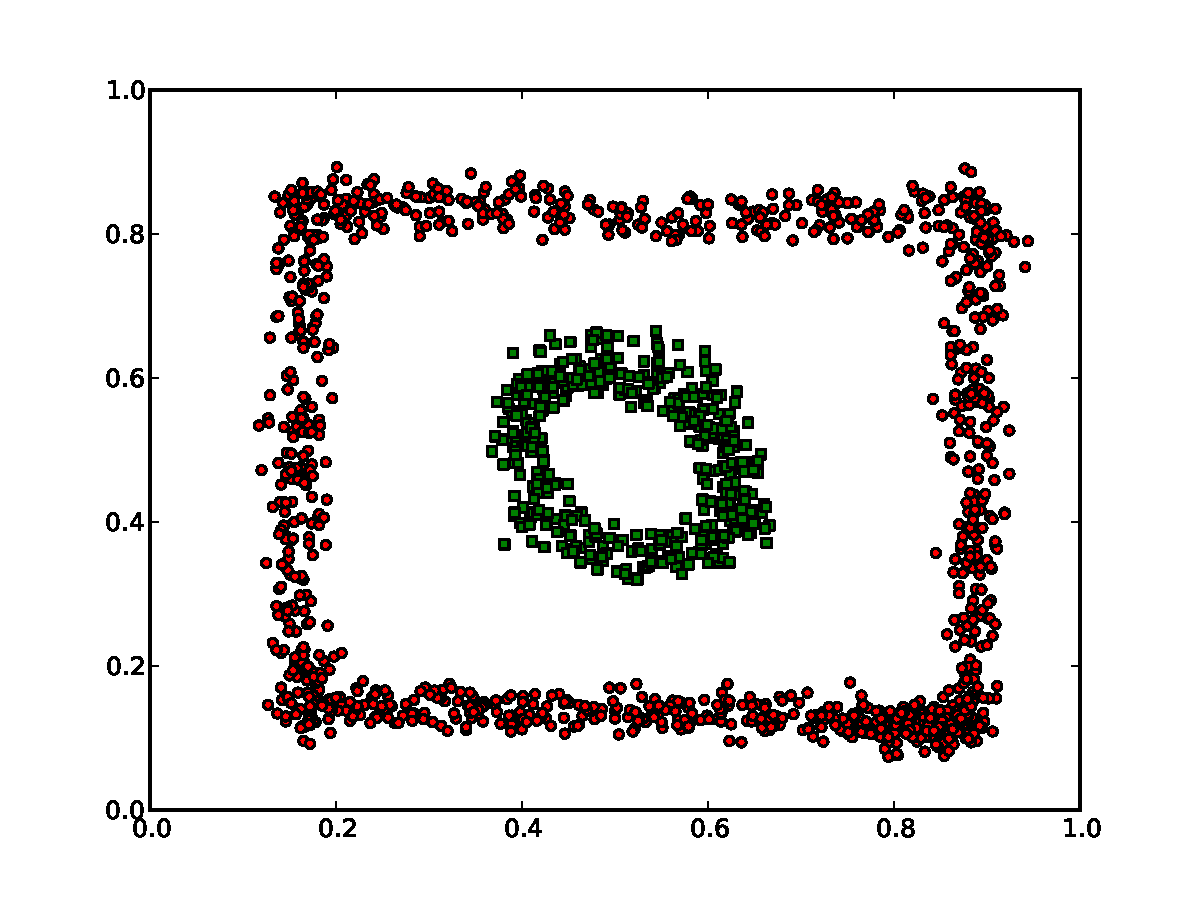
\includegraphics[width=15pc]{circle-weird.pdf}
\caption{Dataset named ''nested-circle''.}
\label{dataset2}
\end{figure}

\begin{figure}[ht]
\centering
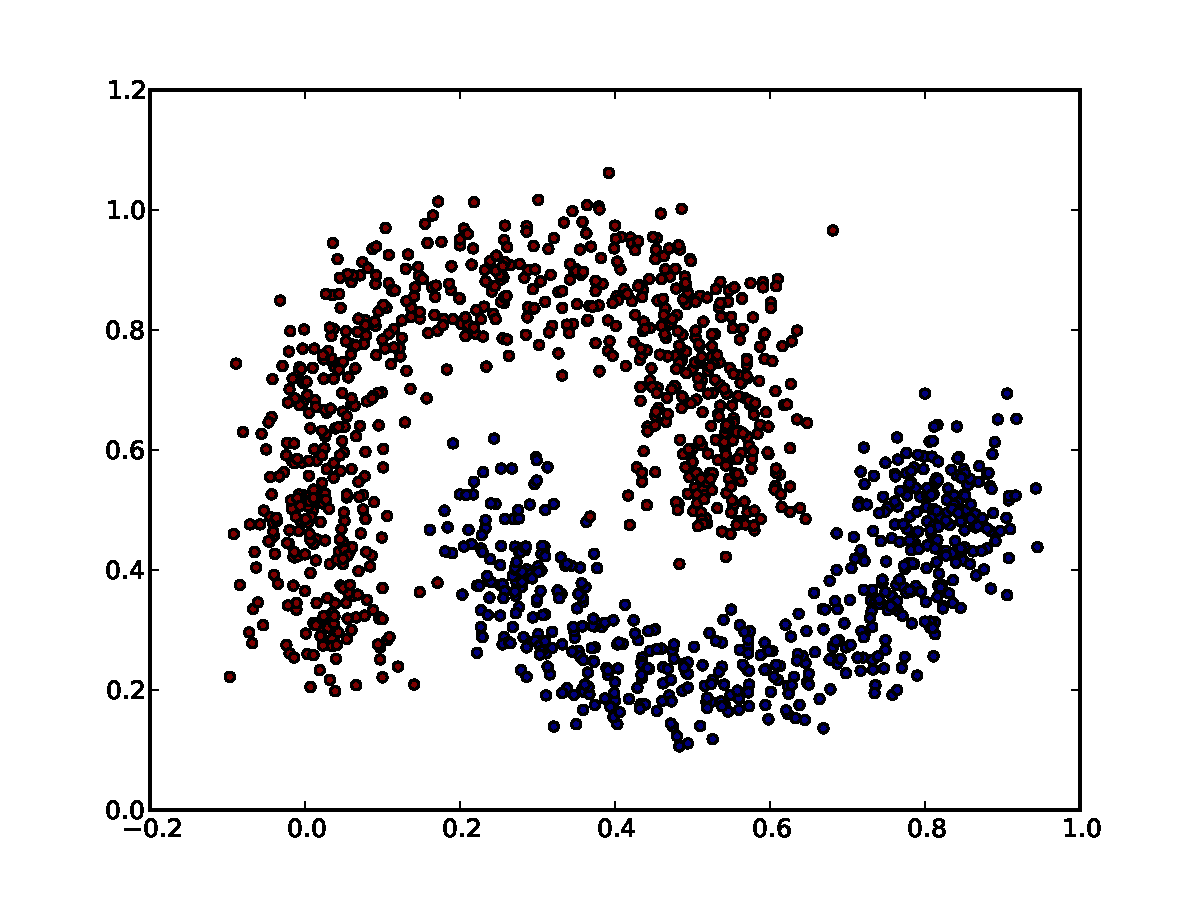
\includegraphics[width=15pc]{half-moons.pdf}
\caption{Dataset named ''half-moons''.}
\label{dataset3}
\end{figure}

\FloatBarrier


\subsection{Red-Blue}

As this was a simple problem all algorithms proved to be successful as we can see in table \ref{redblueresults}. In this
dataset the worst was DBSCAN. The reason is that DBSCAN is detecting noise as well.

\begin{figure}[th]
\centering
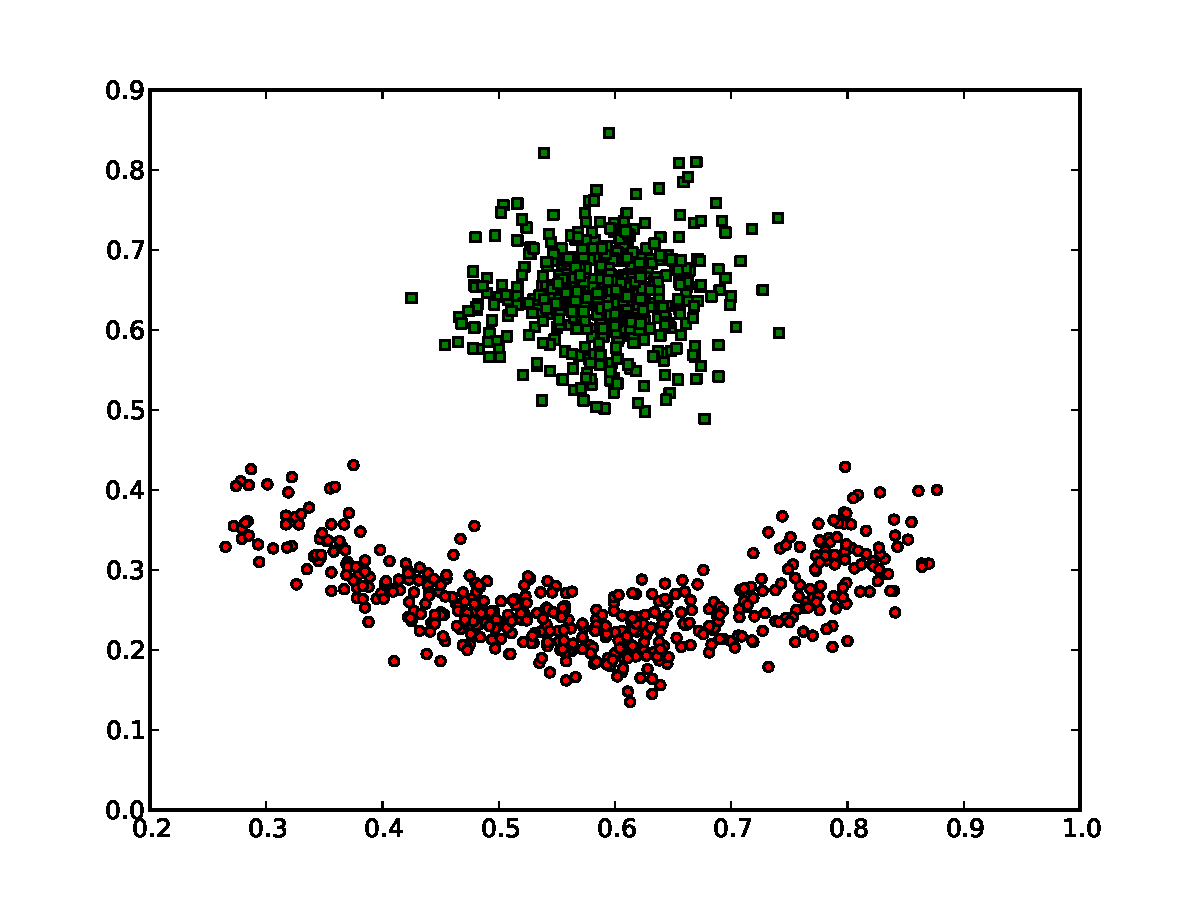
\includegraphics[width=15pc]{ECMC_red-blue-clusters.pdf}
\caption{ECMC on red-blue.}
\label{ECMC_redblue}
\end{figure}

\begin{figure}[th]
\centering
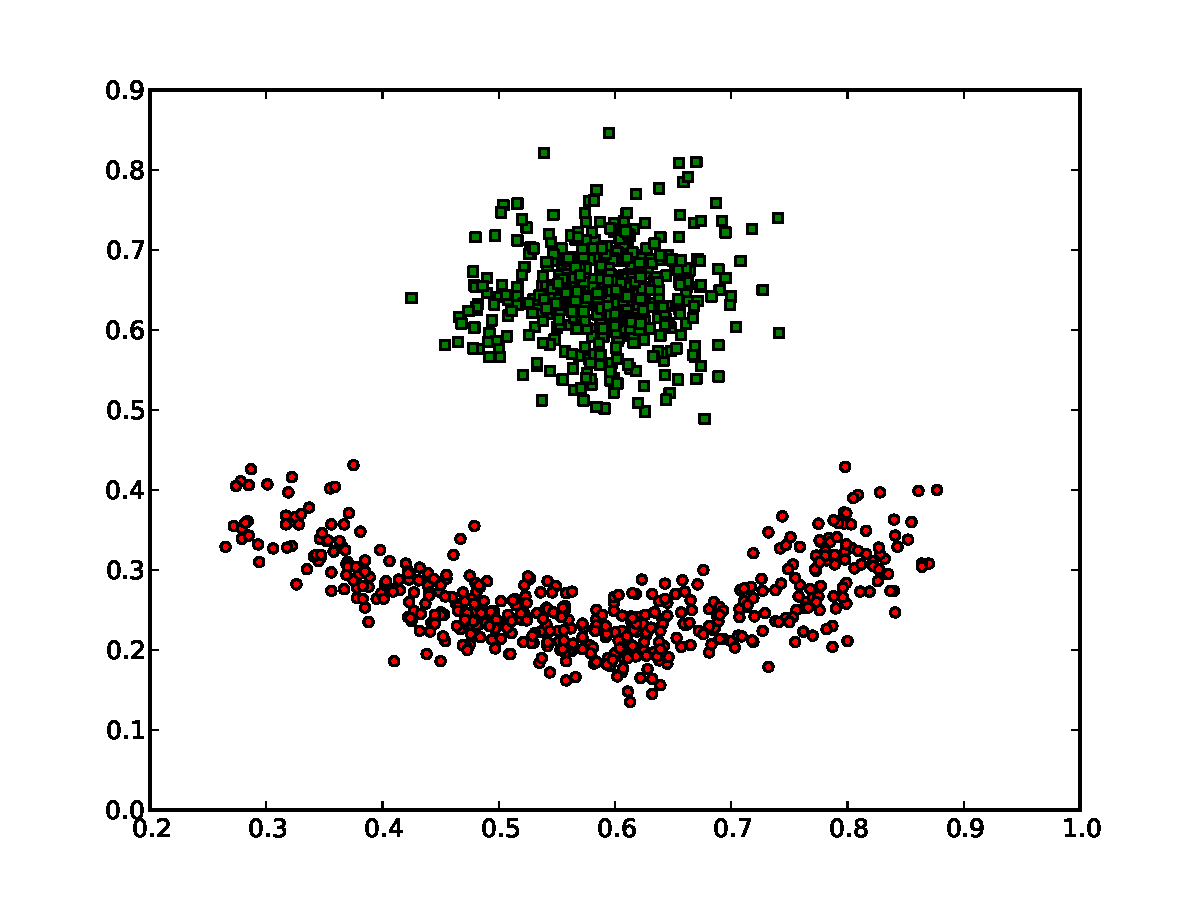
\includegraphics[width=15pc]{GMM_red-blue-clusters.pdf}
\caption{GMM on red-blue.}
\label{GMM_redblue}
\end{figure}

\begin{figure}[th]
\centering
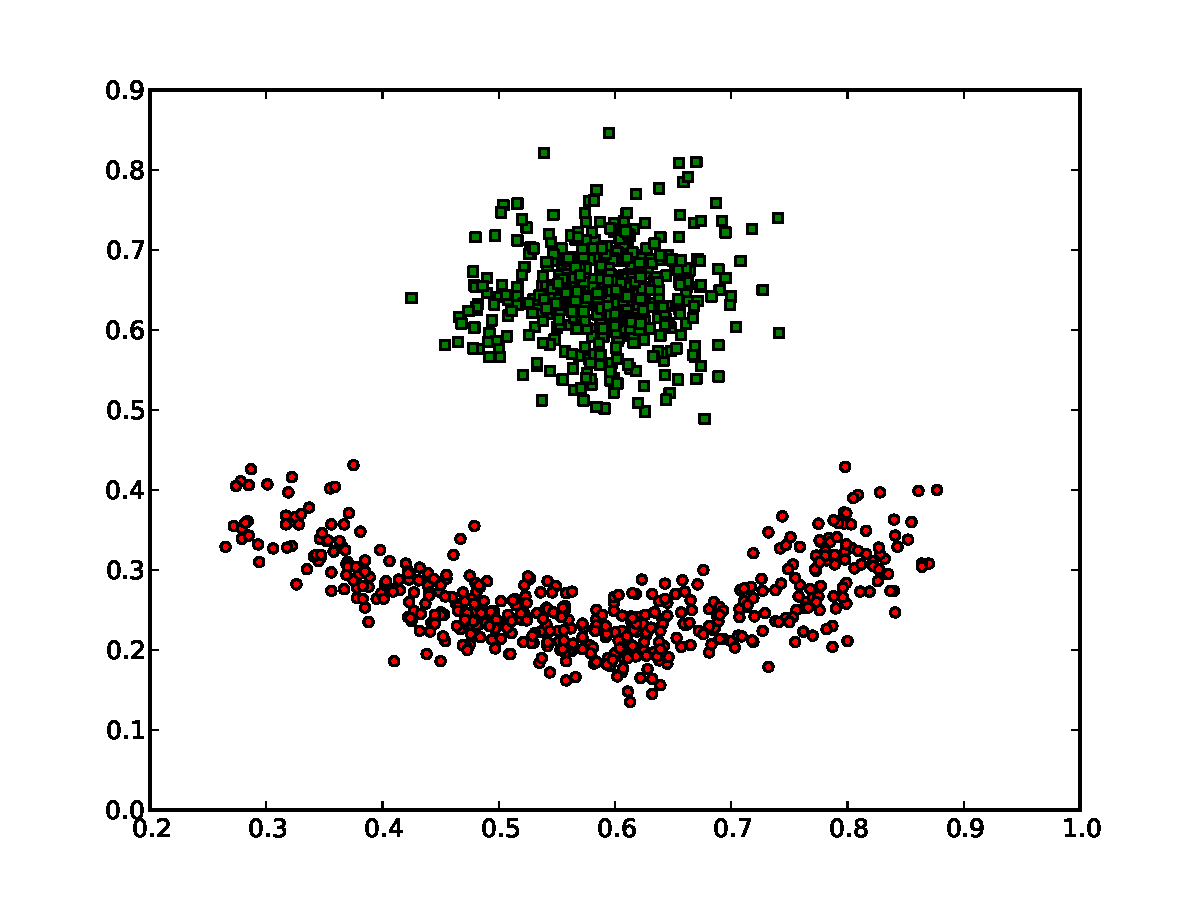
\includegraphics[width=15pc]{spectral_red-blue-cluster.pdf}
\caption{Spectral clustering on red-blue.}
\label{spectral_redblue}
\end{figure}

\begin{figure}[th]
\centering
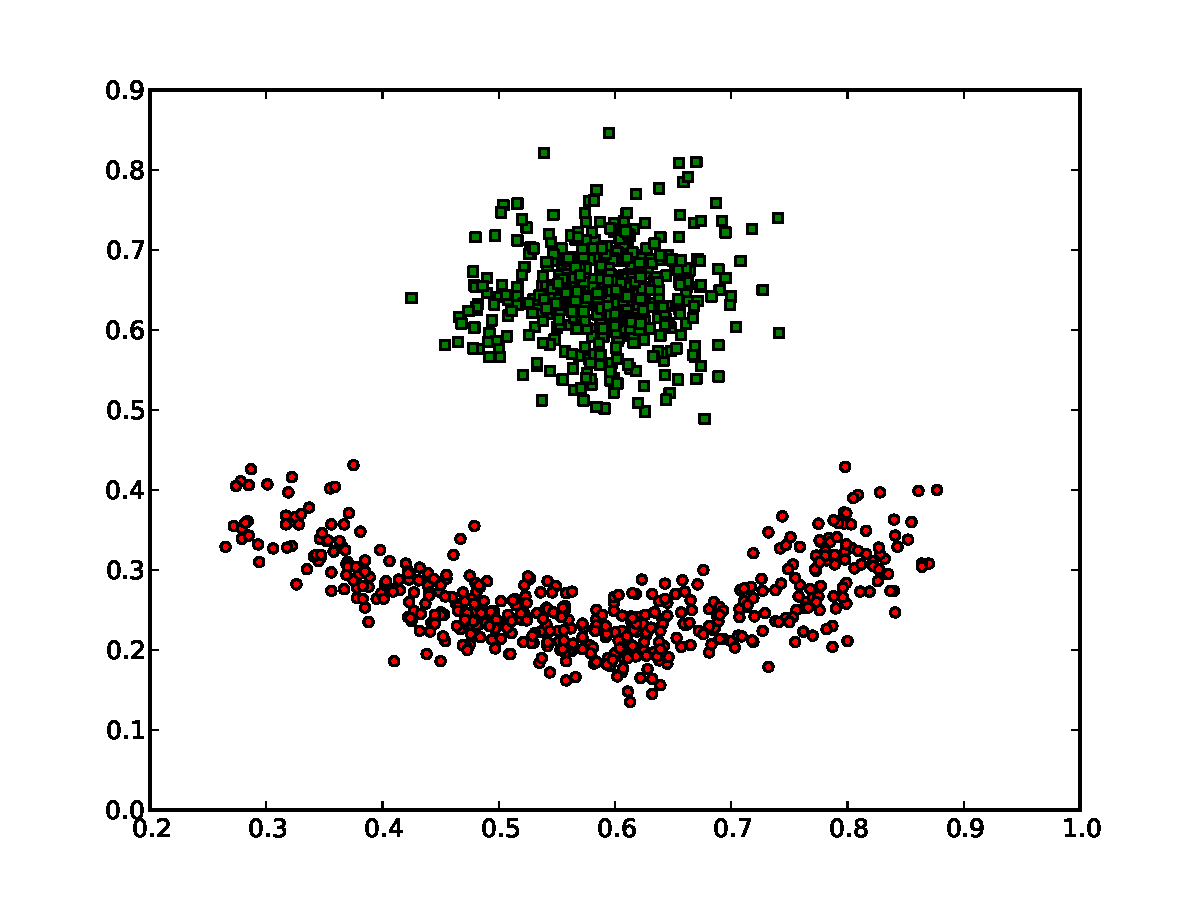
\includegraphics[width=15pc]{kmeans_red-blue-clusters.pdf}
\caption{k-means clustering on red-blue.}
\label{kmeans_redblue}
\end{figure}

\begin{figure}[th]
\centering
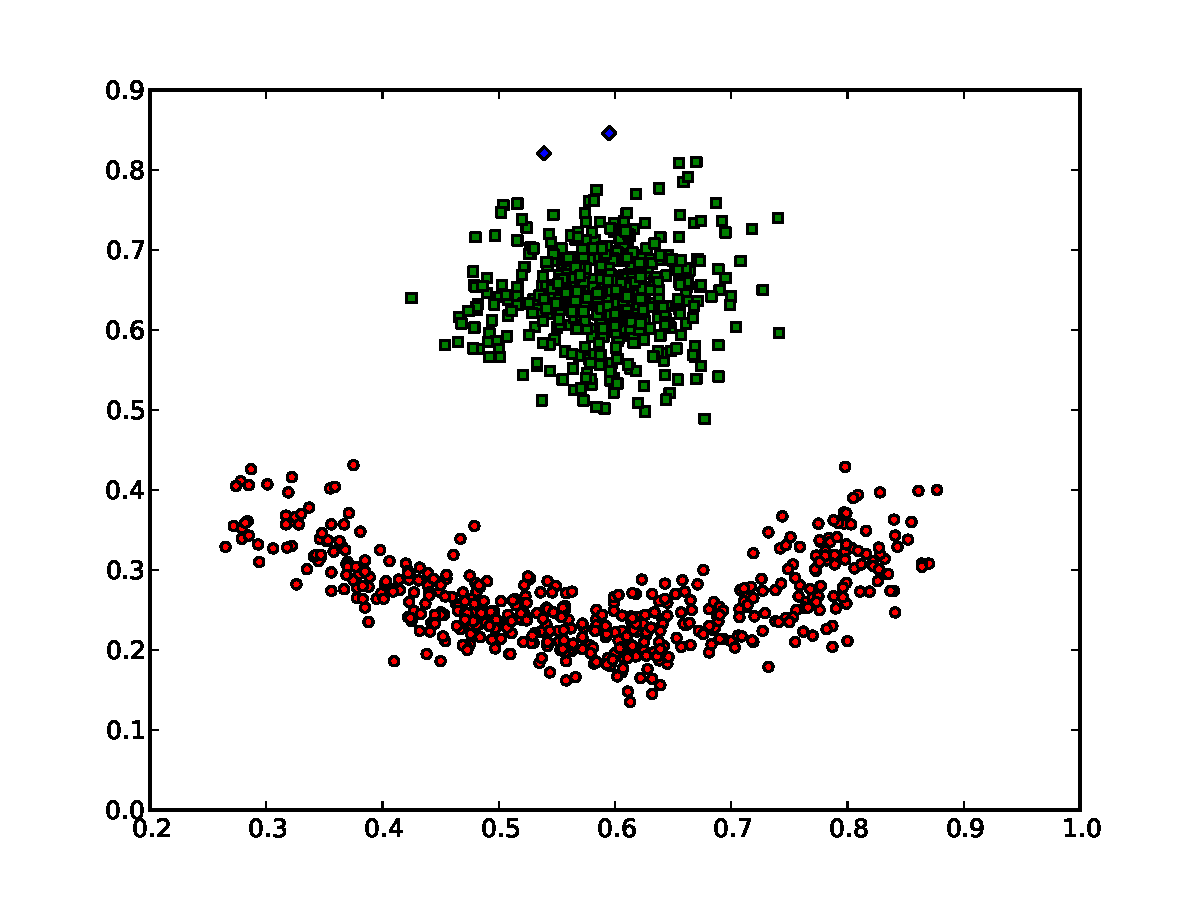
\includegraphics[width=15pc]{dbscan_red-blue-clusters.pdf}
\caption{DBSCAN on red-blue.}
\label{DBSCAN_redblue}
\end{figure}

\begin{table}[htbp]
\caption{Results for red-blue-clusters.}
\label{redblueresults}
\begin{center}
\setlength{\tabcolsep}{3pt}
\begin{tabular}{ |c|c|c|c|c| }
\hline
	Algorithm & ARI & Homogeneity & Completeness & V-measure\\ \hline
	
	ECMC & 1.000 & 1.000 & 1.000 & 1.000 \\ \hline
	GMM & 1.000 & 1.000 & 1.000 & 1.000 \\ \hline
	Spectral & 0.998 & 0.989 & 1.000 & 0.995 \\ \hline
	k-means & 1.000 & 1.000 & 1.000 & 1.000 \\ \hline
	DBSCAN & 0.996 & 0.981 & 1.000 & 0.990 \\ \hline
\end{tabular}
\end{center}
\end{table}


\subsection{Nested circle}
This dataset as described is more difficult to be clustered and the outcome are bad results for most of
the algorithms. As we can see in table \ref{circleweirdresults} the only algorithm that managed
to get good result is DBSCAN.

\begin{figure}[th]
\centering
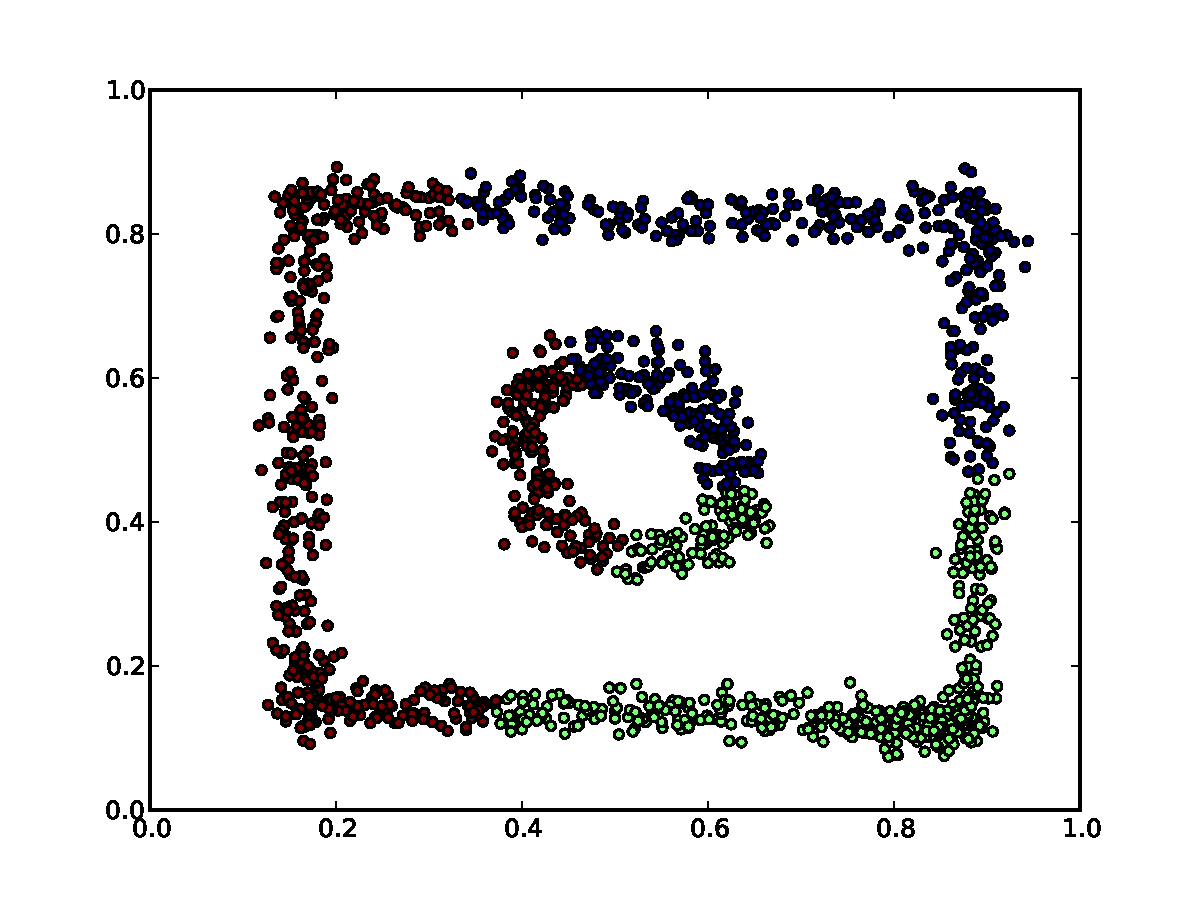
\includegraphics[width=15pc]{ECMC_circle-weird.pdf}
\caption{ECMC on nested-circle.}
\label{ECMC_circleweird}
\end{figure}

\begin{figure}[th]
\centering
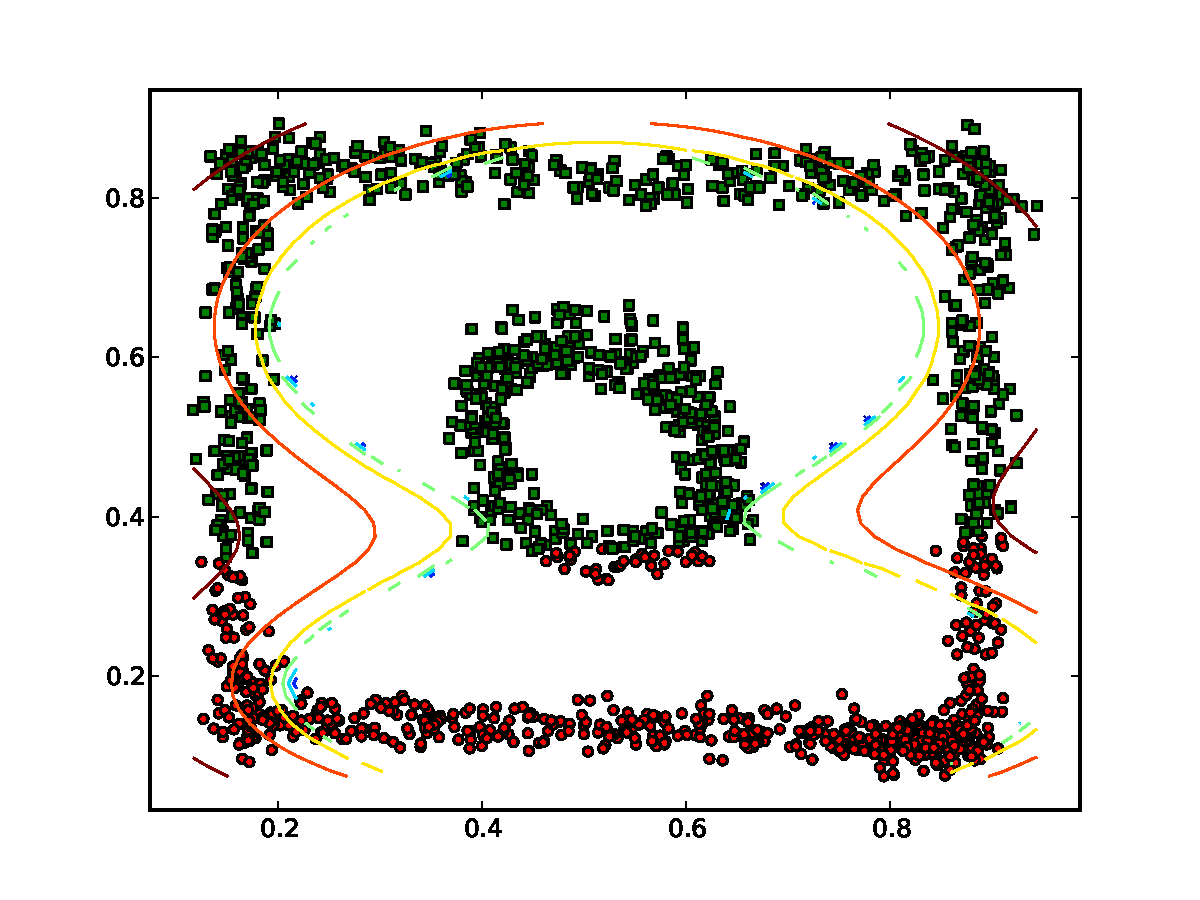
\includegraphics[width=15pc]{GMM_circle-weird.pdf}
\caption{GMM on nested-circle.}
\label{GMM_circleweird}
\end{figure}

\begin{figure}[th]
\centering
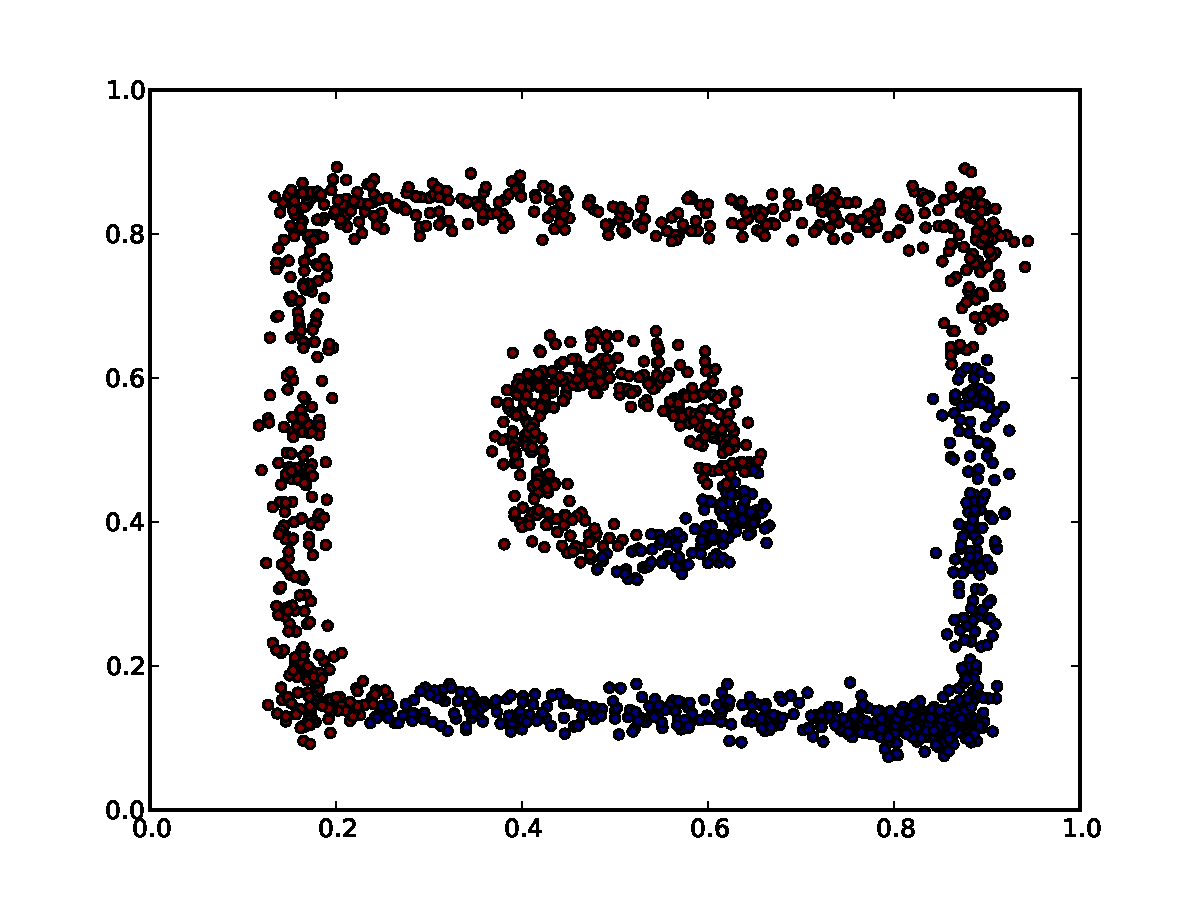
\includegraphics[width=15pc]{spectral_circle-weird.pdf}
\caption{Spectral clustering on nested-circle.}
\label{spectral_circleweird}
\end{figure}

\begin{figure}[th]
\centering
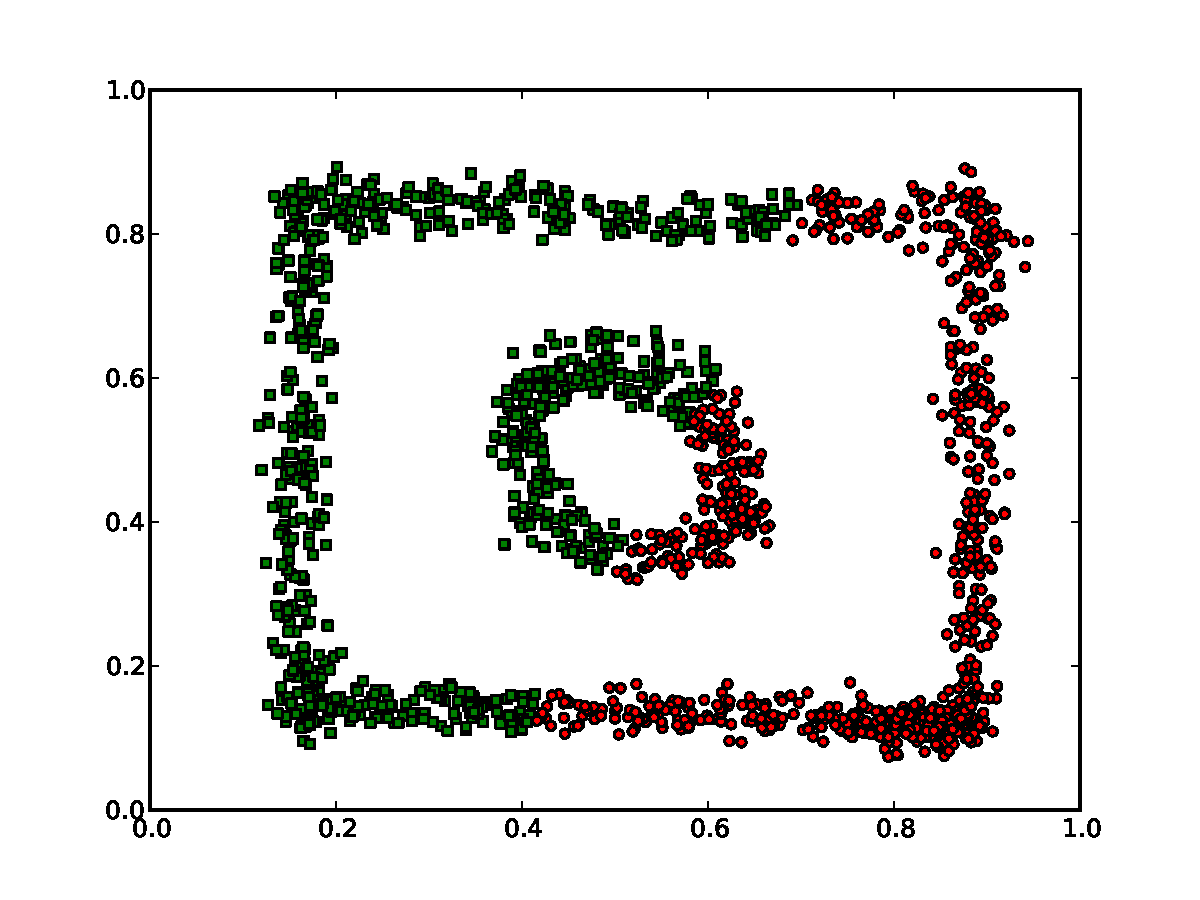
\includegraphics[width=15pc]{kmeans_circle-weird.pdf}
\caption{k-means clustering on nested-circle.}
\label{kmeans_circleweird}
\end{figure}

\begin{figure}[th]
\centering
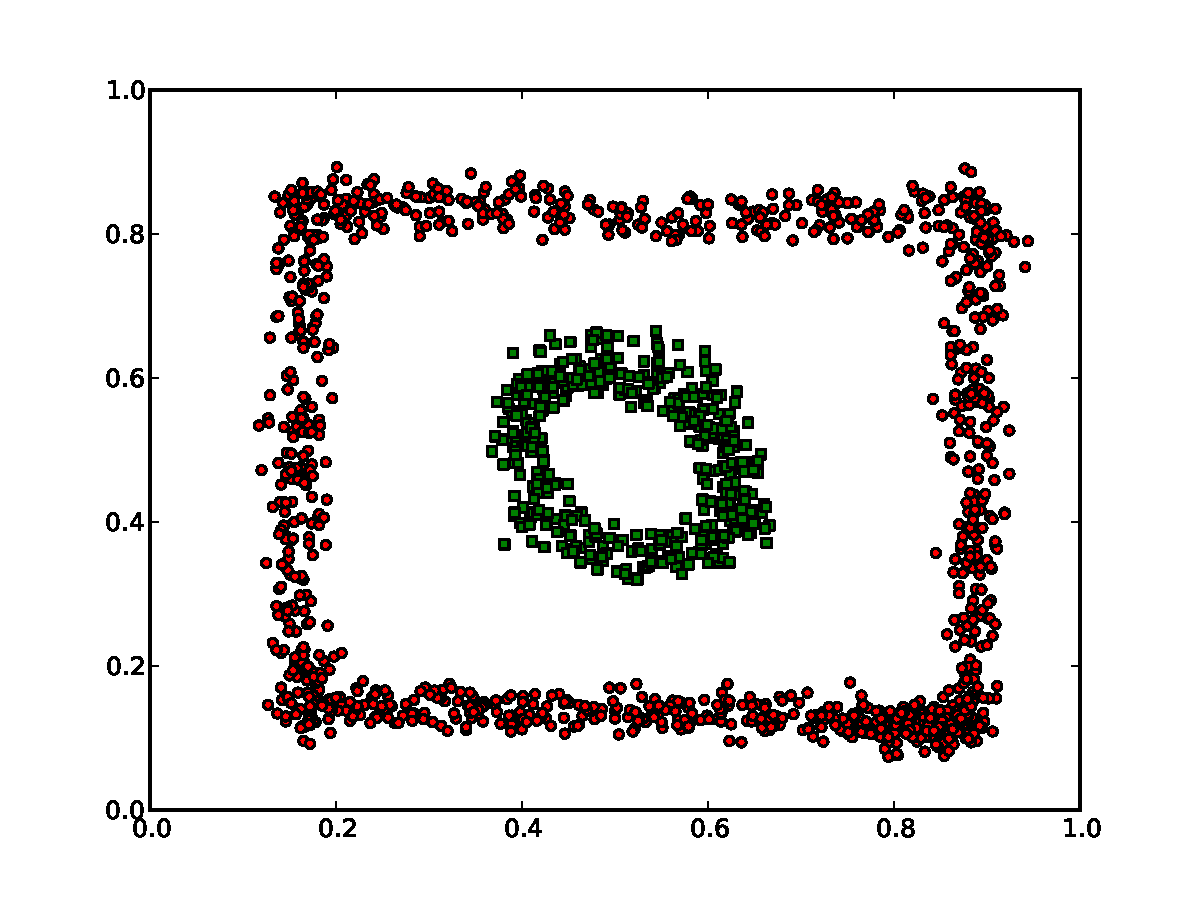
\includegraphics[width=15pc]{dbscan_circle-weird.pdf}
\caption{DBSCAN on nested-circle.}
\label{DBSCAN_circleweird}
\end{figure}

\begin{table}[htbp]
\caption{Results for nested-circle.}
\label{circleweirdresults}
\begin{center}
\setlength{\tabcolsep}{3pt}
\begin{tabular}{ |c|c|c|c|c| }
\hline
	Algorithm & ARI & Homogeneity & Completeness & V-measure\\ \hline
	
	ECMC & 0.012 & 0.011 & 0.013 & 0.012 \\ \hline
	GMM & 0.011 & 0.016 & 0.019 & 0.017 \\ \hline
	Spectral & 0.002 & 0.031 & 0.036 & 0.033 \\ \hline
	k-means & 0.013 & 0.012 & 0.014 & 0.013 \\ \hline
	DBSCAN & 1.000 & 1.000 & 1.000 & 1.000 \\ \hline
\end{tabular}
\end{center}
\end{table}


\subsection{Half-moons}

This dataset showed also as difficult, however algorithms still did better here as in ''wierd circle'' dataset. Again
the best one was DBSCAN as we can see in table \ref{halfmoonsresults}. 

\begin{figure}[th]
\centering
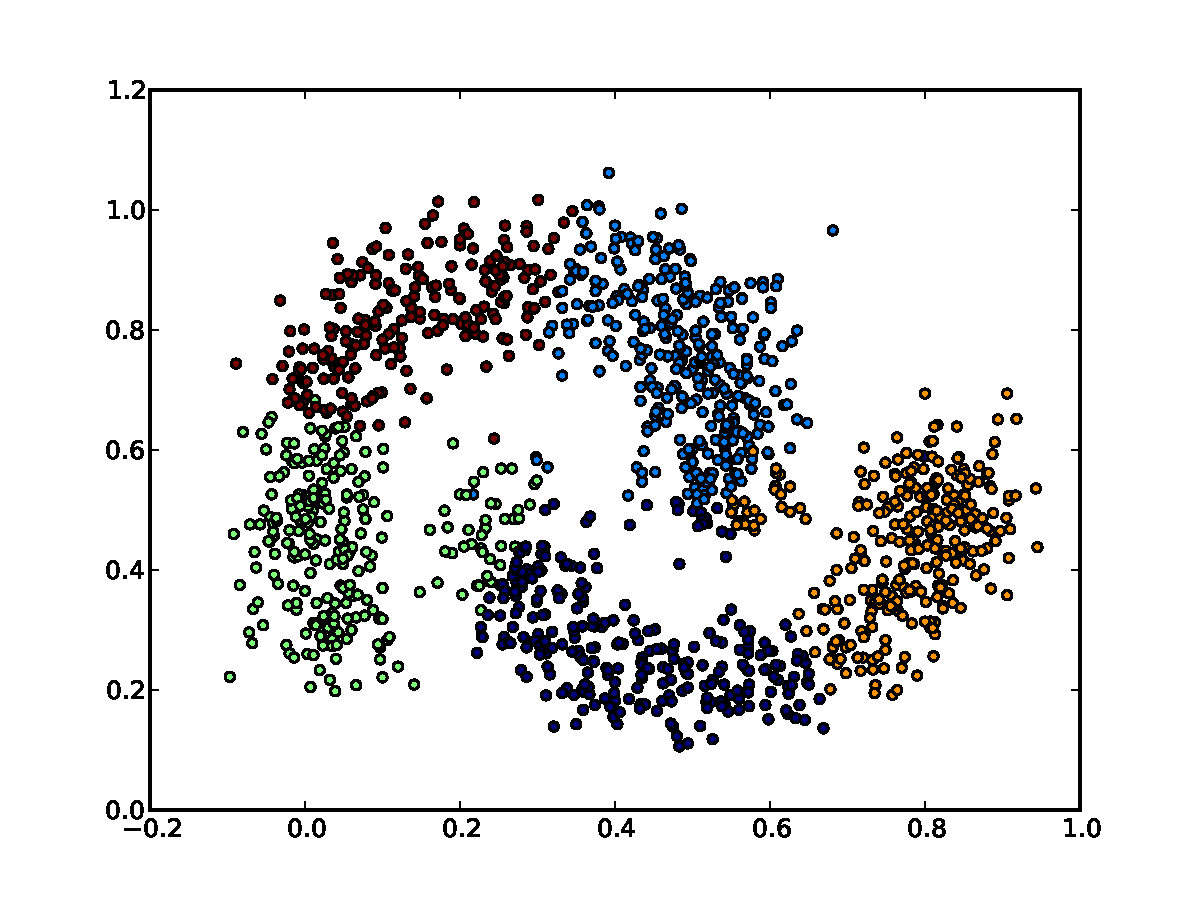
\includegraphics[width=15pc]{ECMC_half-moons.pdf}
\caption{ECMC on half-moons.}
\label{ECMC_halfmoons}
\end{figure}

\begin{figure}[th]
\centering
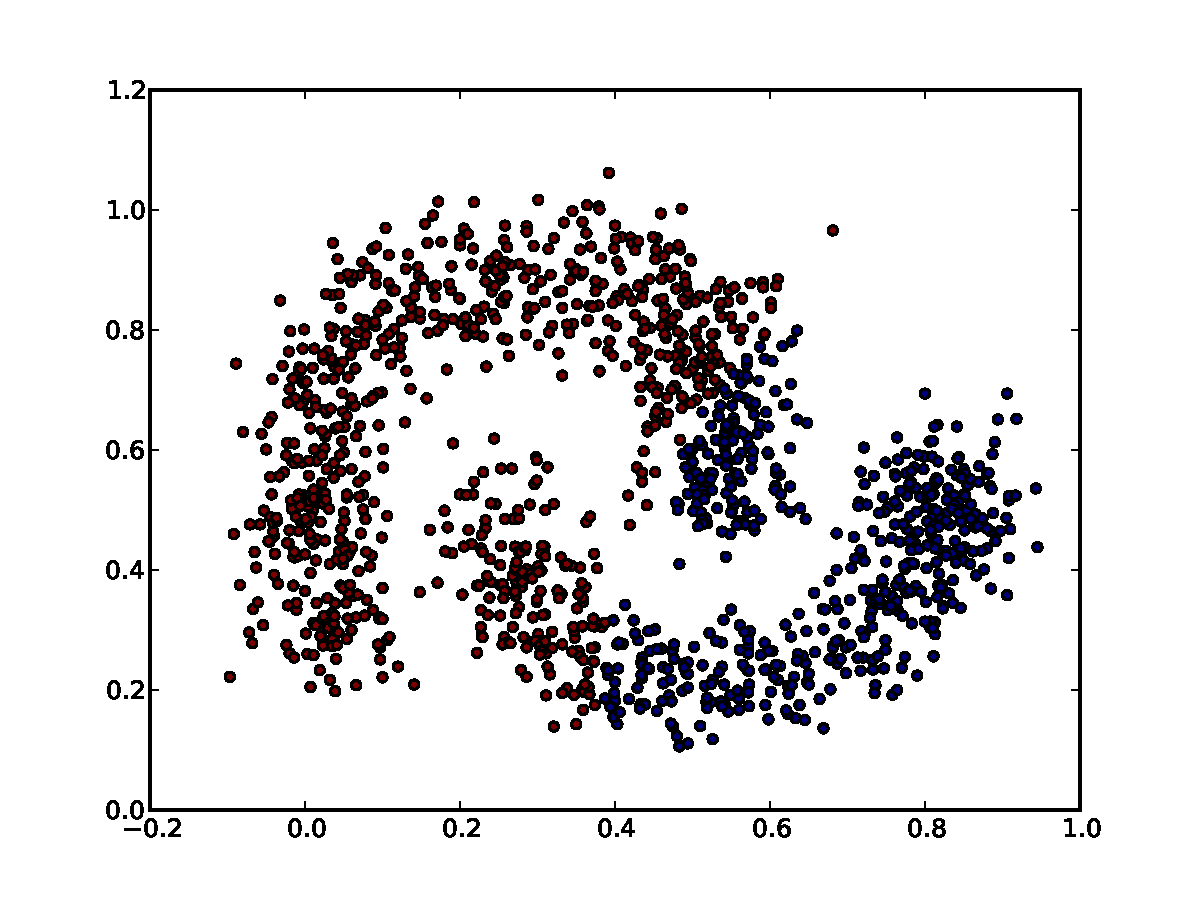
\includegraphics[width=15pc]{GMM_half-moons.pdf}
\caption{GMM on half-moons.}
\label{GMM_halfmoons}
\end{figure}

\begin{figure}[th]
\centering
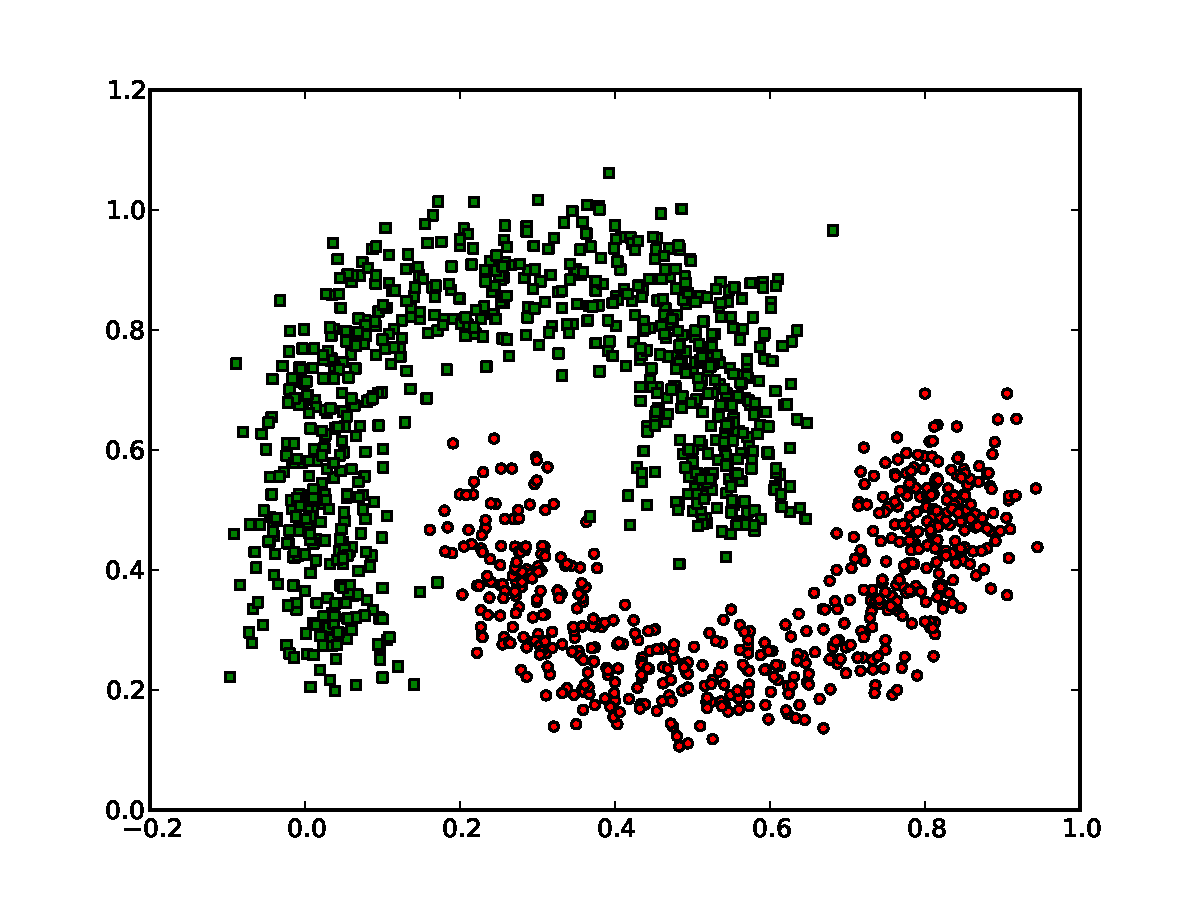
\includegraphics[width=15pc]{spectral_half-moons.pdf}
\caption{Spectral clustering on half-moons.}
\label{spectral_halfmoons}
\end{figure}

\begin{figure}[th]
\centering
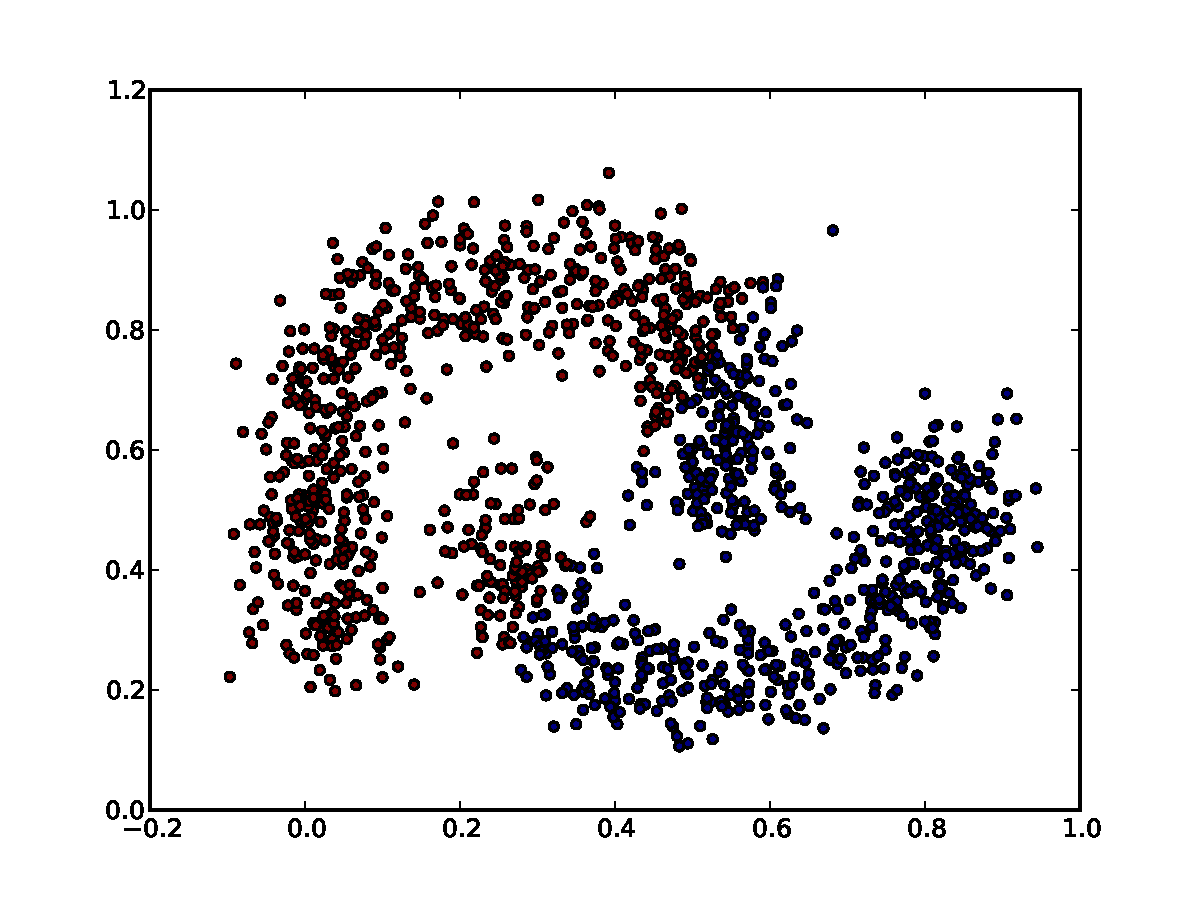
\includegraphics[width=15pc]{kmeans_half-moons.pdf}
\caption{k-means clustering on half-moons.}
\label{kmeans_halfmoons}
\end{figure}

\begin{figure}[th]
\centering
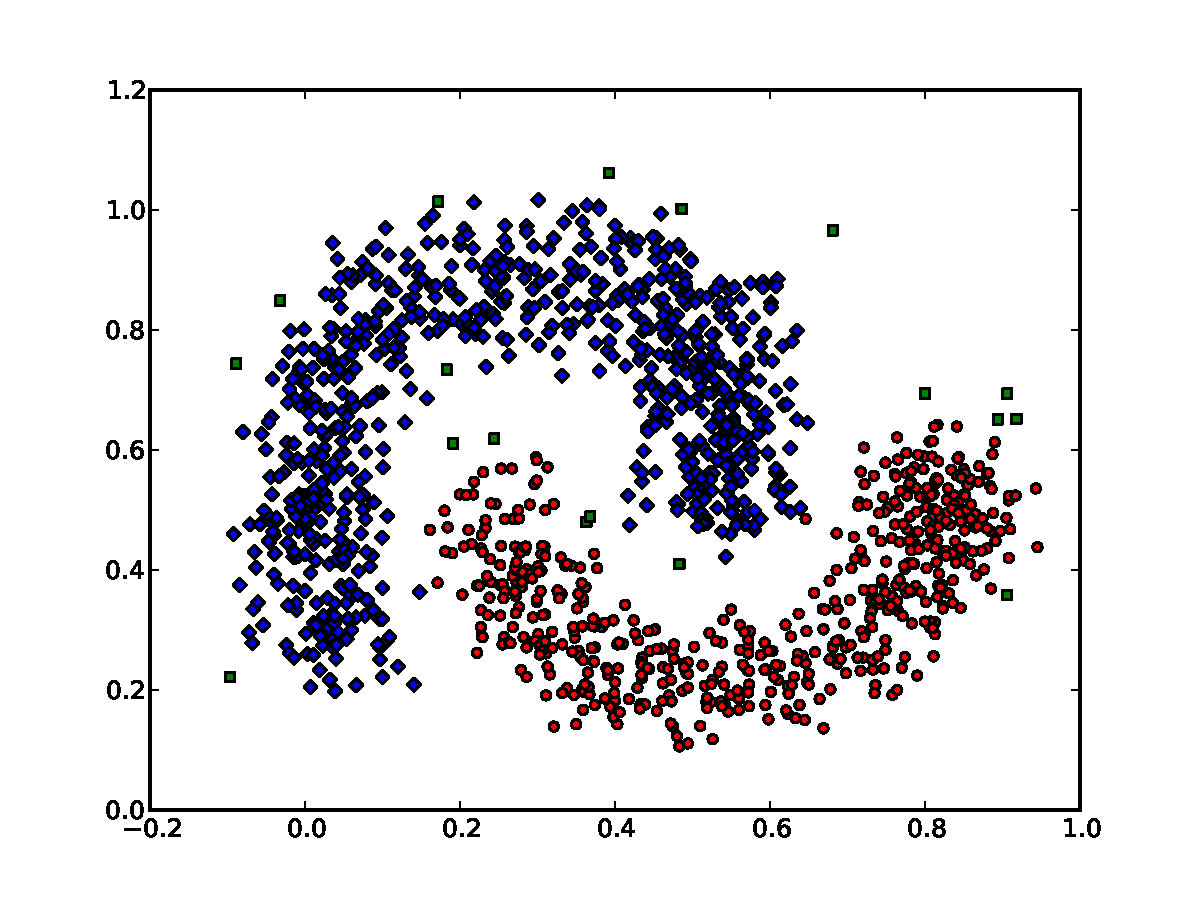
\includegraphics[width=15pc]{dbscan_half-moons.pdf}
\caption{DBSCAN on half-moons.}
\label{DBSCAN_halfmoons}
\end{figure}

\begin{table}[htbp]
\caption{Results for half-moons.}
\label{halfmoonsresults}
\begin{center}
\setlength{\tabcolsep}{3pt}
\begin{tabular}{ |c|c|c|c|c| }
\hline
	Algorithm & ARI & Homogeneity & Completeness & V-measure\\ \hline
	
	ECMC & 0.329 & 0.258 & 0.262 & 0.260 \\ \hline
	GMM & 0.325 & 0.243 & 0.239 & 0.241 \\ \hline
	Spectral & 0.259 & 0.202 & 0.207 & 0.204 \\ \hline
	k-means & 0.343 & 0.268 & 0.273 & 0.271 \\ \hline
	DBSCAN & 0.967 & 0.890 & 0.972 & 0.929 \\ \hline
\end{tabular}
\end{center}
\end{table}


\section{Conclusions}

As we can see results show us that DBSCAN is one of the best algorithm. The only place others
could beat it was with the simpliest datasets where it's advantage of detecting noise really showed
as disadvantage.

Even though DBSCAN showed as the best algorithm overall every task of clustering should be
considered as a problem of it's own. Research should be done which of algorithms
really fits it best.

\section*{Acknowledgements}
The authors wish to thank the mentor for all his help and suggestions.

\bibliographystyle{ieeetr}
\bibliography{references}
%\section*{References}
%\begin{thebibliography}{9}

%\bibitem{jaindubes88}
    %A. K. Jain, R. C. Dubes,
    %\emph{Algorithms for Clustering Data,}
    %Prentice Hall,
    %Englewood Cliffs, NJ,
    %1988.

%\bibitem{jenssen05}
    %R. Jenssen,
    %\emph{An Information Theoretic Approach to Machine Learning},
    %2005

%\bibitem{kononenko07}
    %I. Kononenko,
    %\emph{Machine Learning and Data Mining: Introduction to Principles and Algorithms},
    %Horwood,
    %2007

%\bibitem{vmeasure}
    %A. Rosenberg, J. Hirschberg,
    %\emph{V-Measure: A Conditional Entropy-Based External Cluster Evaluation Measure},
    %In Proceedings of the 2007 Joint Conference on Empirical Methods in Natural Language Processing and Computational Natural Language Learning Prague (2007), pp. 410-420.

%\bibitem{ecm}
    %Q. Song, N. Kasabov,
    %\emph{ECM - A Novel On-line, Evolving Clustering Method and Its Applications},

%\end{thebibliography}

\end{document}
